\documentclass[aspectratio=169,11pt]{beamer}
\usepackage[UTF8,fontset=none]{ctex}
\setCJKmainfont{Microsoft JhengHei}
\setCJKsansfont{Microsoft JhengHei}
\usepackage{amsmath,amssymb,booktabs,array}
\usepackage{pgfplots}
\pgfplotsset{compat=1.18}
\definecolor{navy}{HTML}{183750}
\definecolor{teal}{HTML}{007E87}
\definecolor{orange}{HTML}{B45A20}
\setbeamercolor{normal text}{fg=navy,bg=white}
\setbeamercolor{structure}{fg=teal}
\setbeamercolor{frametitle}{fg=navy}
\setbeamercolor{alerted text}{fg=orange}
\setbeamerfont{frametitle}{size=\Large,series=\bfseries}
\setbeamertemplate{navigation symbols}{}
\setbeamertemplate{itemize items}[circle]
\setbeamersize{text margin left=8mm,text margin right=8mm}
\setbeamertemplate{footline}{\hspace{8mm}\scriptsize Handout 3 自讀筆記\hfill\insertsectionhead\hfill\insertframenumber/\inserttotalframenumber\hspace{8mm}\vspace{3mm}}
\newcommand{\src}[1]{\par\vfill{\scriptsize\color{teal}#1}}
\newcommand{\slide}[3]{\begin{frame}[t]{#1}#3\src{#2}\end{frame}}
\newcommand{\bi}{\begin{itemize}\setlength{\itemsep}{5pt}}
\newcommand{\ei}{\end{itemize}}
\newcommand{\key}[1]{\par\medskip{\color{teal}\bfseries #1}\par\smallskip}
\newcommand{\dd}{\mathrm{d}}
\newcommand{\bookslide}[3]{\slide{#1}{課本：#2。頁碼為書本印刷頁碼}{#3}}
% Original images extracted losslessly from the supplied textbook PDF.
\newcommand{\originalfigure}[6]{
\begin{frame}[t]{課本原圖 #1：#2}
\centering
\includegraphics[width=.94\linewidth,height=5.05cm,keepaspectratio]{figures/#4}\par
\vspace{2mm}\raggedright\small #5\par
\vfill{\scriptsize\color{teal}原圖：Collinson, 第 3 版，Fig. #1，p. #3。#6}\par
\end{frame}}


\newcommand{\handoutfigure}[3]{
\begin{frame}[t]{講義原頁 #1：#2}
\centering
\includegraphics[width=.97\linewidth,height=5.65cm,keepaspectratio]{figures/#3}\par
\vfill{\scriptsize\color{teal}原圖與文字：賴盈誌老師提供之 Handout，PDF 第 #1 頁。}\par
\end{frame}}
\title{基礎氣動與縱向靜穩定}
\subtitle{Handout 3\\繁體中文自讀詳解}
\author{依賴盈誌老師課程講義整理}
\date{CA7528 Digital Avionics\quad Fall 2026}
\begin{document}
\begin{frame}\titlepage\centering\small 概念、原圖、推導、算例與自我檢查\end{frame}
\section{閱讀地圖}
\slide{範圍與閱讀方式}{Handout 3，PDF pp. 1--65}{
\bi
\item Handout 3 與既有 Chapter 3 的氣動、配平、穩定性自讀詳解。
\item 原頁碼一律指講義 PDF 頁序。標示「課本」的頁碼則是 Collinson 第三章印刷頁碼。
\item 先讀概念，再對照原圖。自我檢查先遮住參考解答，再獨立計算或口頭說明。
\item 自編算例與補充推導依題內假設使用。歷史機型、服務與表格依原教材背景理解。
\ei
}
\slide{分次閱讀安排}{Handout 3 閱讀地圖}{
\small
\bi
\item \textbf{講義導讀}：FMS、Autopilot 與 FBW 的層級。
\item \textbf{講義術語}：力的方向與飛行角度。
\item \textbf{講義核對}：升力與失速的閱讀限制、配平力矩與參考幾何、中性點與靜裕度的定義。
\item \textbf{整合檢查}：自然穩定與受控穩定。
\ei
}
\slide{公式推導與詳解閱讀地圖}{Collinson 第三章對應主題；課本頁碼於各頁標示}{
\small
\bi
\item 3.2 基礎空氣動力學：壓力、升阻力係數、失速、算例、氣動中心與配平。
\item 3.3 飛機穩定性：恢復力矩、靜穩定與動穩定、中性點、靜裕度及不穩定配置。
\item 講義核對與自我檢查：整合各個定義，重新計算並檢查近似條件。
\ei
}
\section{講義導讀}
\slide{FMS、Autopilot 與 FBW 的層級}{Handout 3，PDF pp. 1--7；概念整理與補充推導}{
\small
\bi
\item FMS 支援航路與飛行管理，Autopilot 執行所選的飛行目標，FBW 處理操縱命令與底層控制。
\item 較外層以任務與航路為目標，較內層以姿態、角速度及操縱面反應為目標。
\item 副翼、升降舵、方向舵是基本操縱面，複合操縱面可能同時支援多軸或不同功能。
\ei
\key{閱讀重點}先辨認控制層級，再從飛機受力、配平與穩定性理解底層控制需求。
}
\handoutfigure{3}{FMS、Autopilot 與 FBW 的層級}{handout03-p003.png}
\handoutfigure{6}{FMS、Autopilot 與 FBW 的層級}{handout03-p006.png}
\slide{自我檢查：FMS、Autopilot 與 FBW 的層級}{依 Handout 範圍自編問題與參考解答}{
\small
\key{先自行作答}
為什麼 FBW 需要比 FMS 航路管理更快的回授？
\key{參考解答}
內層需要及時處理飛機運動與擾動，外層處理較慢的航路目標。兩層若頻寬配置不當，會產生追蹤與穩定性問題。
}
\section{講義術語}
\slide{力的方向與飛行角度}{Handout 3，PDF pp. 8--13；概念整理與補充推導}{
\small
\bi
\item 升力垂直相對氣流，阻力與相對氣流平行，重量沿重力方向，推力依發動機安裝方向。
\item 只有在指定條件下，才能說升力向上或與重量大小相等。
\item 迎角、俯仰姿態及航跡角使用不同參考線，航向與地面航跡也可能因風而不同。
\ei
\key{閱讀重點}後續筆記採機體 x 向前、y 向右、z 向下，角度單位一律在公式附近確認。
}
\handoutfigure{11}{力的方向與飛行角度}{handout03-p011.png}
\handoutfigure{12}{力的方向與飛行角度}{handout03-p012.png}
\slide{自我檢查：力的方向與飛行角度}{依 Handout 範圍自編問題與參考解答}{
\small
\key{先自行作答}
自編算例：縱向平面中 $\theta=8^\circ$、$\gamma=3^\circ$，機體基準與翼弦一致，迎角為多少？
\key{參考解答}
$\alpha\simeq\theta-\gamma=5^\circ$。若翼弦另有固定安裝角，還需把安裝角納入關係。
}
\section{3.2 基礎空氣動力學}
\bookslide{升力與阻力的兩種描述}{3.2.1，pp. 101--103}{
\bi
\item 壓力觀點：翼面各處壓力分布與表面剪應力，積分後形成合力。教材以翼上減壓、翼下增壓作直觀說明。
\item 動量觀點：機翼使流過的空氣改變動量，空氣對機翼施加反作用力。
\item 兩種觀點描述同一個氣動作用，不能把它們當成兩份可相加的升力來源。
\item 升力垂直於相對氣流，阻力沿相對氣流方向，與飛機相對空氣的運動方向相反。
\ei
\key{閱讀提醒}教材的「上表面約占三分之二」是示意比例，不能套用到所有翼型、迎角與飛行條件。
}
\originalfigure{3.1}{翼面壓力分布}{102}{fig-3-01.png}{比較上、下翼面的壓力分布，並將分布力連到合升力。}{}

\originalfigure{3.2}{氣流動量與反作用力}{102}{fig-3-02.png}{觀察氣流偏轉與動量改變，這與壓力分布是同一氣動作用的兩種描述。}{}

\bookslide{迎角、姿態與航跡角}{3.2.2，p. 103；角度關係為補充}{
\bi
\item 迎角（angle of attack），$\alpha$：翼弦基準線與相對氣流方向的夾角。
\item 教材用 angle of incidence 表示迎角。其他資料中的 incidence 也可能指機翼安裝角。
\item 俯仰角 $\theta$ 表示機體姿態，航跡角 $\gamma$ 表示速度向量相對水平面的方向。
\ei
\[\alpha\simeq\theta-\gamma\]
此式假設縱向平面運動，且翼弦與機體基準線一致。若有固定安裝角，必須另行計入。
\key{例子}抬頭姿態不保證正在爬升。飛機可能在很大的迎角下仍然下降。
}
\originalfigure{3.3}{迎角、升力與阻力方向}{103}{fig-3-03.png}{迎角以翼弦與相對氣流為基準，升力方向未必等於機體向上方向。}{}

\bookslide{動壓與氣動係數}{3.2.3，p. 104，式 (3.1)--(3.5)}{
\[Q=\frac12\rho V_T^2,\qquad L_W=QS C_L,\qquad D_W=QS C_D\]
\bi
\item $\rho$：空氣密度，$\mathrm{kg/m^3}$。$V_T$：相對空氣的速度，$\mathrm{m/s}$。
\item $Q$：動壓，單位 $\mathrm{Pa=N/m^2}$。$S$：機翼參考面積，$\mathrm{m^2}$。
\item $C_L,C_D$ 無因次，包含翼型、迎角與流況等影響。力的大小由動壓、面積與係數共同決定。
\item 保留大寫 $Q$ 表示動壓，避免與俯仰角速度 $q$ 混淆。
\ei
\key{適用限制}可壓縮流的衝壓差不直接等於 $\frac12\rho V_T^2$，但動壓仍可用此式定義。
}
\bookslide{升力曲線與失速}{3.2.3，pp. 104--105}{
\[C_L\simeq C_{L0}+C_{L\alpha}\alpha
       =C_{L\alpha}(\alpha-\alpha_{L=0})\]
\bi
\item 失速前的一段迎角範圍可近似線性。斜率 $C_{L\alpha}$ 必須註明每度或每弧度。
\item 超過臨界迎角後，分離流使升力曲線不再遵守線性式，不能繼續外插。
\item 教材典型值：一般翼型 $C_{L\max}\approx1.2$--$1.6$，臨界迎角約 $15^\circ$--$20^\circ$，三角翼可更高。
\item 失速與迎角有關。所謂失速速度，還依重量、密度、載荷因數與構型而變。
\ei
}
\originalfigure{3.4}{升阻力係數與迎角}{105}{fig-3-04.png}{注意失速附近的升力曲線轉折，以及大迎角下阻力的增加。}{}

\bookslide{阻力極線與高升力裝置}{3.2.3，pp. 104--106，式 (3.6)}{
\[C_D\simeq C_{D0}+kC_L^2\]
\bi
\item $C_{D0}$ 表示此模型中與升力平方項分離的基礎阻力，$kC_L^2$ 描述隨升力增加的阻力。
\item 需要更大的 $C_L$ 時，阻力通常增加，維持速度就需要更多推力。
\item 前緣縫翼、前緣襟翼與後緣襟翼改變翼型／流動，增加可用升力。教材列舉高升力構型 $C_{L\max}$ 可達約 3--4。
\item 接近音速時，壓縮性會明顯改變 $C_L,C_D$。不可用同一組低速係數涵蓋整個飛行包線。
\ei
}
\originalfigure{3.5}{前緣縫翼與後緣襟翼}{106}{fig-3-05.png}{比較高升力裝置伸出與收回時，升力係數對迎角的變化。}{}

\bookslide{等速平飛與低速限制}{3.2.3--3.2.4，pp. 104--107；補充推導}{
忽略尾翼分擔、推力垂直分量等因素，等速平飛近似有
\[L\simeq mg,\quad T\simeq D,\quad
C_{L,\mathrm{req}}=\frac{2mg}{\rho V_T^2S}.\]
\bi
\item 同一重量與密度下，速度減半，需要的 $C_L$ 增為四倍。
\item 密度降低時，維持相同真空速與升力需要更高的 $C_L$。
\item 可用升力係數存在上限，因此 $V_s=\sqrt{2mg/(\rho S C_{L\max})}$。
\ei
\key{補充}載荷因數為 $n=L/(mg)$ 時，在同一構型與密度下，$V_{s,n}=V_{s,1}\sqrt n$。
}
\bookslide{教材算例：低空低速的迎角}{3.2.4，pp. 105--107}{
\small
已知 $m=30{,}000\ \mathrm{kg}$，$S=75\ \mathrm{m^2}$，$\rho=1.225\ \mathrm{kg/m^3}$，$V_T=80\ \mathrm{m/s}$。
\[Q=\tfrac12(1.225)(80)^2=3920\ \mathrm{Pa}\]
\[C_L=\frac{30{,}000(9.81)}{3920(75)}=1.001\approx1.0\]
教材特別假設升力曲線通過原點，且 $C_{L\max}=1.2$ 對應 $\alpha_{\max}=15^\circ$。
\[C_{L\alpha}=\frac{1.2}{15}=0.08/\mathrm{deg},\qquad
\alpha\approx\frac{1.0}{0.08}=12.5^\circ\]
\key{意義}這個低速平飛條件已接近教材設定的臨界迎角，進一步增加升力的餘裕有限。
}
\bookslide{教材算例：速度與可用機動加速度}{3.2.4，pp. 106--107}{
\small
同一低空密度，改為 $200\ \mathrm{m/s}$ 平飛：
\[\alpha\approx12.5^\circ\left(\frac{80}{200}\right)^2=2.0^\circ.\]
高度 $30{,}000\ \mathrm{ft}$，$\rho=0.4583$，$V_T=225\ \mathrm{m/s}$：
\[L_{\max}=\tfrac12(0.4583)(225)^2(75)(1.2)
\approx1.044\times10^6\ \mathrm{N}.\]
\[n_{\max}=\frac{L_{\max}}{mg}\approx3.55,\qquad
\frac{L_{\max}-mg}{m}\approx25.0\ \mathrm{m/s^2}\approx2.55g.\]
\key{兩個不同量}3.55 是升力／重量的載荷因數。2.55$g$ 是此算例扣除重力後的向上淨加速度。教材的「2.5$g$」指後者。
}
\bookslide{壓力中心與氣動中心}{3.2.5，pp. 107--108}{
\bi
\item 壓力中心（centre of pressure）：合氣動力的作用位置，關於此點的合力矩為零。位置隨迎角改變。
\item 氣動中心（aerodynamic centre, AC）：在所考慮條件下，關於此點的俯仰力矩對迎角變化近似不變。
\item 使用 AC 可把機翼等效為作用於固定位置的氣動力，加上一個近似固定的俯仰偶矩。
\item 教材的近似位置：亞音速約四分之一翼弦，超音速趨近二分之一翼弦。整機 AC 與單獨機翼 AC 必須區分。
\ei
\[M_0=QSc C_{M0},\qquad [QSc]=\mathrm{N\,m}.\]
}
\bookslide{尾翼如何平衡俯仰力矩}{3.2.6，pp. 108--110，式 (3.9)--(3.12)}{
採教材圖 3.6 的配置，$x>0$ 表示機翼升力作用點在 CG 後方，$L_t>0$ 表示向下的尾翼力大小，$M_0>0$ 表示低頭偶矩大小。
\[M=-L_Wx-M_0+L_tl_t,\qquad L_t=k_tQS_t C_{Lt}\]
\[C_M=-\frac{x}{c}C_L-C_{M0}
       +k_t\frac{S_tl_t}{Sc}C_{Lt}.\]
\bi
\item 尾翼向下作用時，關於 CG 產生抬頭力矩，抵銷其他低頭力矩。
\item $k_t$ 為尾翼處動壓／自由流動壓，教材典型範圍 0.65--0.95。
\item $S_tl_t$ 稱尾翼容積，$S_tl_t/(Sc)$ 為無因次尾翼容積比。
\ei
}
\originalfigure{3.6}{主翼與尾翼的配平作用}{108}{fig-3-06.png}{依 CG、機翼氣動中心與尾翼力臂，逐項核對力矩正負號。}{}

\bookslide{配平的代價與幾何量提醒}{3.2.5--3.2.6，pp. 108--110}{
\bi
\item 向下尾翼力使總向上升力減少。因此主翼需提供 $L_W=mg+L_t$，而非只提供 $mg$。
\item 尾翼面積或力臂增大，通常可增加控制力矩與恢復作用，但會付出重量、阻力等代價。
\item 配平只要求合力與合力矩滿足指定運動。穩定性要另外檢查受擾後的變化率。
\ei
\key{核對提醒：平均翼弦}教材以 $c=S/b$ 作簡化。一般非矩形機翼的平均氣動弦長（MAC）不必等於 $S/b$。本章算式使用給定的參考弦長 $c$，不把此簡化當作通則。
}
\originalfigure{3.7}{機翼與尾翼力矩的疊加}{110}{fig-3-07.png}{合成曲線的零點決定配平迎角，斜率則反映靜恢復作用。}{}


\section{3.3 飛機穩定性}
\bookslide{靜穩定與動穩定}{3.3，pp. 110--111}{
\small
\begin{tabular}{p{.18\textwidth}p{.65\textwidth}}
\toprule 類型 & 要觀察的量\\\midrule
靜穩定 & 受擾後，初始力或力矩是否朝恢復平衡的方向？\\
靜中性 & 受擾後沒有一階恢復力／力矩，也沒有一階發散趨勢。\\
靜不穩定 & 初始力或力矩使偏離程度增加。\\
動穩定 & 完整時間響應是否衰減回到平衡？需考慮慣性、阻尼與耦合。\\\bottomrule
\end{tabular}
\key{重要區分}有恢復力矩不代表振盪一定衰減。若阻尼不足或為負，系統仍可能持續振盪或動態發散。
\key{配平與穩定}配平決定平衡點的位置，穩定性決定平衡點附近的行為。
}
\originalfigure{3.8}{穩定、中性與不穩定的類比}{110}{fig-3-08.png}{比較小球離開平衡位置後，受到的作用是否促使它回到原處。}{}

\originalfigure{3.9(a)}{靜穩定的初始趨勢}{111}{fig-3-09a.png}{分別觀察初始恢復趨勢，以及時間響應的振幅是否衰減。}{}

\originalfigure{3.9(b)}{動穩定的振幅變化}{111}{fig-3-09b.png}{分別觀察初始恢復趨勢，以及時間響應的振幅是否衰減。}{}

\bookslide{縱向靜穩定判據}{3.3.1，pp. 110--112}{
抬頭力矩為正。在配平迎角 $\alpha_T$ 附近作線性展開：
\[C_M(\alpha)\simeq C_M(\alpha_T)+C_{M\alpha}(\alpha-\alpha_T).\]
\[\boxed{C_M(\alpha_T)=0,\qquad C_{M\alpha}<0}\]
\bi
\item 若迎角增加，需產生負的低頭力矩，將迎角拉回。
\item 若迎角減少，需產生正的抬頭力矩，將迎角拉回。
\item $C_{M\alpha}=0$ 對應一階靜中性。$C_{M\alpha}>0$ 表示縱向靜不穩定。
\ei
}
\originalfigure{3.10}{俯仰力矩係數的斜率}{112}{fig-3-10.png}{原圖同時比較正、零、負斜率，對應不同的縱向靜穩定情況。}{}

\bookslide{靜穩定曲線的讀法}{3.3.1，圖 3.10；下圖為概念示意}{
\begin{columns}[T]
\begin{column}{.56\textwidth}
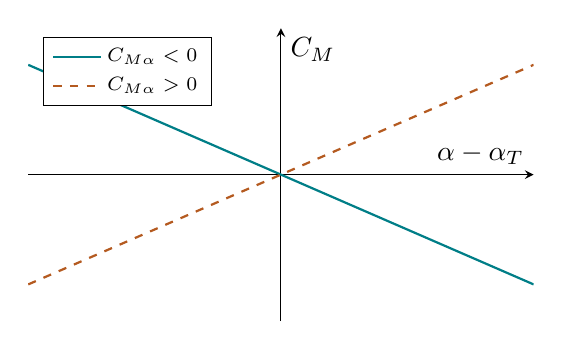
\begin{tikzpicture}
\begin{axis}[width=8cm,height=5.3cm,xlabel={$\alpha-\alpha_T$},ylabel={$C_M$},axis lines=middle,xmin=-3,xmax=3,ymin=-1,ymax=1,xtick={0},ytick={0},legend style={font=\scriptsize,at={(.03,.97)},anchor=north west}]
\addplot[teal,thick,domain=-3:3]{-.25*x};\addlegendentry{$C_{M\alpha}<0$}
\addplot[orange,thick,dashed,domain=-3:3]{.25*x};\addlegendentry{$C_{M\alpha}>0$}
\end{axis}
\end{tikzpicture}
\end{column}
\begin{column}{.4\textwidth}
\bi\item 零力矩交點表示配平。
\item 斜率表示初始恢復能力。
\item 更陡的負斜率通常代表更大的靜恢復作用。
\item 此圖沒有時間軸，不能直接讀取阻尼或收斂時間。\ei
\end{column}
\end{columns}
}
\bookslide{中性點與靜裕度}{3.3.1，pp. 111--112}{
\[SM=\frac{x_{NP}-x_{CG}}{c}\]
此處位置沿機身向後為正。$NP$ 為使 $C_{M\alpha}=0$ 的 CG 位置，也稱中性點。
\bi
\item CG 在中性點前方：$SM>0$，對應教材的縱向靜穩定配置。
\item CG 向後移動，靜裕度下降。越過中性點就失去自然縱向靜穩定。
\item 教材例子：$SM=10\%$、$c=4\ \mathrm{m}$，CG 往後移 $0.4\ \mathrm{m}$ 會到達中性點。
\ei
\key{補充關係}簡化線性模型中，$C_{M\alpha}=-C_{L\alpha}SM$。升力斜率與中性點必須對應同一整機模型及操縱面約束。
}
\originalfigure{3.11}{陣風與自然恢復力矩}{113}{fig-3-11.png}{比較向上陣風、配平及向下陣風時，迎角與恢復力矩的方向。}{}

\bookslide{不穩定配置與主動穩定}{3.3.2，pp. 112--114}{
\bi
\item 教材比較的配置將 CG 放在整機氣動中心後方，尾翼可向上提供配平升力。
\item 主翼所需升力減少，迎角與升力相關阻力可能下降。尾翼容積也可能縮小，但仍受起飛旋轉等要求限制。
\item 代價是失去自然恢復趨勢，需要感測器、計算器和致動器持續閉迴路控制。
\item 教材指出高機動不穩定戰機的擾動振幅倍增時間可能短至約 0.25 秒，超過飛行員可持續補償的能力。
\ei
\key{補充計算}若振幅按 $e^{\lambda t}$ 增長，$t_2=\ln2/\lambda$。$t_2=0.25\ \mathrm{s}$ 對應 $\lambda\approx2.77\ \mathrm{s^{-1}}$。
}
\originalfigure{3.12}{不穩定飛機的配平配置}{113}{fig-3-12.png}{注意 CG 與氣動中心的相對位置，以及尾翼升力的方向。}{}

\originalfigure{3.13}{倒著騎自行車的控制類比}{114}{fig-3-13.png}{教材用此圖說明不穩定配置需要快速、持續的修正。}{}

\originalfigure{3.14}{Tornado 與 FBW Jaguar}{115}{fig-3-14.png}{教材以編隊照片比較配平尾翼力方向不同的兩種配置。}{Photo: Arthur Gibson / British Aerospace Defence Ltd.}

\bookslide{整機穩定性不只由機翼決定}{3.3.3，p. 114；本單元自我檢查}{
\bi
\item 機身也產生升力與側向力，力的作用位置會影響俯仰與偏航穩定性。
\item 吊艙式發動機外罩也可能產生顯著氣動力，不能只把它當作重量。
\item 分析需要使用整機導數，不能直接以孤立機翼資料替代。
\ei
\key{自我檢查}
\begin{enumerate}
\item $C_M=0$ 足以判定穩定？\quad\textbf{否，還須看斜率與完整動態。}
\item CG 後移通常如何影響靜裕度？\quad\textbf{使其減小。}
\item 更大的負 $C_{M\alpha}$ 保證較大阻尼？\quad\textbf{否，恢復與阻尼是不同作用。}
\end{enumerate}
}

\section{講義核對}
\slide{升力與失速的閱讀限制}{Handout 3，PDF pp. 14--37；概念整理與補充推導}{
\small
\bi
\item 壓力積分與動量改變描述同一作用，不能分別計算後再重複相加。
\item 動壓與速度平方成正比，速度增加兩倍使動壓增加四倍。
\item 升力曲線的線性近似只適用於限定範圍。失速後升力不必變成零。
\item 講義中的上、下翼面比例及臨界迎角屬示意或典型敘述，實際數值與翼型和流況有關。
\ei
\key{閱讀重點}升力計算須同時核對速度、密度、面積與係數，並確認是否仍在模型適用範圍。
}
\handoutfigure{29}{升力與失速的閱讀限制}{handout03-p029.png}
\handoutfigure{35}{升力與失速的閱讀限制}{handout03-p035.png}
\slide{自我檢查：升力與失速的閱讀限制}{依 Handout 範圍自編問題與參考解答}{
\small
\key{先自行作答}
飛機失速後還有沒有氣動力？為什麼不能繼續用線性升力曲線？
\key{參考解答}
仍有升力、阻力與力矩，但分離流改變係數關係。線性式無法描述該區的變化，必須採用適用的實驗或非線性模型。
}
\slide{配平力矩與參考幾何}{Handout 3，PDF pp. 38--51；概念整理與補充推導}{
\small
\bi
\item 配平要求指定飛行狀態的合力與合力矩平衡，重心、氣動中心及尾翼力臂會影響所需舵角。
\item 壓力中心隨迎角移動，氣動中心用來將氣動力與近似固定偶矩分開表示。
\item 一般非矩形翼的平均氣動弦長與 $S/b$ 不必相同，計算需使用題目指定的基準。
\ei
\key{閱讀重點}力矩係數必須清楚註明作用點、參考面積、參考弦長與正方向。
}
\handoutfigure{42}{配平力矩與參考幾何}{handout03-p042.png}
\handoutfigure{45}{配平力矩與參考幾何}{handout03-p045.png}
\slide{自我檢查：配平力矩與參考幾何}{依 Handout 範圍自編問題與參考解答}{
\small
\key{先自行作答}
若尾翼在重心後方提供向下的力，通常產生抬頭還是低頭力矩？
\key{參考解答}
對一般後置尾翼配置，向下的尾翼力對重心產生抬頭力矩。主翼也需額外提供升力以平衡尾翼下壓力。
}
\slide{中性點與靜裕度的定義}{Handout 3，PDF pp. 52--60；概念整理與補充推導}{
\small
\bi
\item 靜裕度使用全機中性點 $x_{NP}$：$SM=(x_{NP}-x_{CG})/\bar c$。
\item 在常用縱向靜穩定分析中，重心在中性點之前對應正靜裕度。
\item 講義把靜裕度寫成與壓力中心距離的敘述容易混淆，計算應採中性點定義。
\item $C_{M0}>0$ 不是所有飛機都須滿足的獨立普遍判據，還要看基準、控制設定及可用配平範圍。
\ei
\key{閱讀重點}固定操縱位置下，核心局部判據是 $C_{M\alpha}<0$，配平則另要求 $C_M=0$。
}
\handoutfigure{57}{中性點與靜裕度的定義}{handout03-p057.png}
\handoutfigure{60}{中性點與靜裕度的定義}{handout03-p060.png}
\slide{自我檢查：中性點與靜裕度的定義}{依 Handout 範圍自編問題與參考解答}{
\small
\key{先自行作答}
自編算例：$x_{NP}=1.10\,\mathrm m$、$x_{CG}=0.85\,\mathrm m$、$\bar c=2.5\,\mathrm m$，求靜裕度。
\key{參考解答}
$SM=(1.10-0.85)/2.5=0.10=10\%$。若重心移至 $1.15\,\mathrm m$，則 $SM=-2\%$，表示這個局部模型下失去自然靜穩定。
}
\section{整合檢查}
\slide{自然穩定與受控穩定}{Handout 3，PDF pp. 61--65；概念整理與補充推導}{
\small
\bi
\item 不穩定配置可由主動回授穩定，但這使感測、計算、致動與故障處理更加關鍵。
\item 靜穩定描述初始恢復趨勢，動態響應還由慣性、阻尼與耦合決定。
\item 講義的不同響應曲線需要同時比較速度、過衝、振盪與任務需求。
\ei
\key{閱讀重點}能配平、自然靜穩定與閉迴路動穩定是三個不同的檢查項目。
}
\handoutfigure{62}{自然穩定與受控穩定}{handout03-p062.png}
\handoutfigure{64}{自然穩定與受控穩定}{handout03-p064.png}
\slide{自我檢查：自然穩定與受控穩定}{依 Handout 範圍自編問題與參考解答}{
\small
\key{先自行作答}
自編模型 $C_M=0.08-0.90\alpha$，$\alpha$ 用 rad。求配平並判斷靜穩定。
\key{參考解答}
$\alpha_T=0.08/0.90=0.08889\,\mathrm{rad}=5.09^\circ$。斜率為 $-0.90/\mathrm{rad}$，在固定控制設定及該局部模型下具有恢復趨勢，尚不足以判斷動態阻尼。
}
\section{複習與來源}
\slide{整合複述檢查}{Handout 3 全份複習}{
\bi
\item 選一項系統功能，說明輸入、輸出、座標、單位與資料來源。
\item 找出一個公式，逐一解釋每個符號，再說明它使用哪些假設。
\item 選一個故障或誤差，追蹤它如何影響下游功能，以及可以用什麼獨立資訊核對。
\item 重做本份的自我檢查，再對照講義與相關公式。
\ei
}
\slide{來源與後續閱讀}{Handout 3 與隨附教材}{
\small
\bi
\item 主要來源：賴盈誌老師，CA7528 Digital Avionics，Handout 3。原始檔保留於上一層資料夾。
\item 版型與重用內容：既有 Chapter03\_SelfStudy\_LaTeX。Handout 3、4 沿用相關章節及其原圖。
\item 第三章重用內容來源：R. P. G. Collinson，\textit{Introduction to Avionics Systems}，第 3 版。
\item 本筆記的重算、核對與延伸為自讀整理，並非授課教師或出版社正式勘誤。
\item 原圖內來源標示與圖說保留，新增題目與參考解答已另行標明。
\ei
}
\end{document}
